% Fisica 1 - Fabrizio Cei - 06/02/2024
% Corpo Rigido - Pagina 16

\subsection{Moto di puro rotolamento nei corpi a sezione circolare}

Il moto di puro rotolamento avviene nei corpi a sezione circolare o comunque senza spigoli, in modo da impedire urti e scivolamento.

\begin{equation}
\vec{v}_Q = \vec{v}_{CM} + \vec{\omega} \times \vec{r}^*
\end{equation}

% Diagramma: cerchio su superficie con CM, punto Q di contatto, asse z verticale, assi x,y, vettore r* da CM a Q
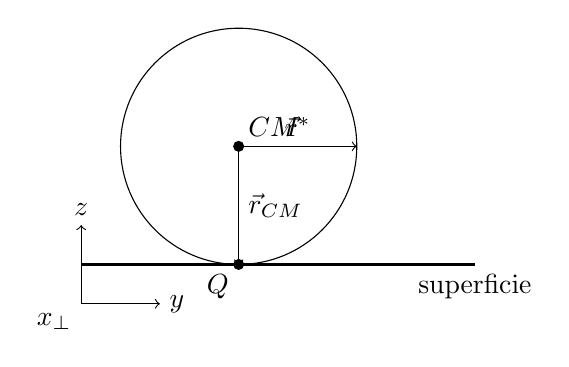
\begin{tikzpicture}
    % Cerchio (sezione del corpo rigido)
    \draw (0,1.5) circle (1.5);
    \fill (0,1.5) circle (2pt) node[above right] {$CM$};
    \fill (0,0) circle (2pt) node[below left] {$Q$};
    \draw[->] (0,1.5) -- (0,0) node[midway, right] {$\vec{r}_{CM}$};
    \draw[->] (0,1.5) -- (1.5,1.5) node[midway, above] {$\vec{r}^*$};
    \draw[thick] (-2,0) -- (3,0) node[below] {superficie};
    % Assi
    \draw[->] (-2,-0.5) -- (-1,-0.5) node[right] {$y$};
    \draw[->] (-2,-0.5) -- (-2,0.5) node[above] {$z$};
    \node[below left] at (-2,-0.5) {$x_\perp$};
\end{tikzpicture}

Se $\vec{v}_{CM} = \vec{\omega} \times (-\vec{r}^*)$, cioè il corpo ruota in senso orario, allora $\vec{v}_Q = 0$, cioè l'asse che passa per $Q$ è \textbf{istantaneamente fermo}.

\begin{itemize}
    \item Inoltre se $\vec{r}^* = \overrightarrow{CM \to Q}$ e $(-\vec{r}^*) = \overrightarrow{Q \to CM}$, allora
\end{itemize}

$\vec{v}_{CM} = \vec{\omega} \times \vec{R}_{Q \to CM}$, cioè $\vec{v}_{CM}$ ruota intorno ad un asse che passa per $Q$, perché $Q$ rispetta (1) e (2). Quindi è l'asse istantaneo di rotazione. Questo si può dimostrare verificando che anche ogni altro punto del corpo rigido ruota attorno a $Q$ ($S$ generico):

\begin{align*}
\vec{v}_S &= \vec{v}_{CM} + \vec{\omega} \times \vec{R}_{CM \to S} = \vec{\omega} \times \vec{R}_{Q \to CM} + \vec{\omega} \times \vec{R}_{CM \to S} \\
&= \vec{\omega} \times (\vec{R}_{Q \to CM} + \vec{R}_{CM \to S}) = \vec{\omega} \times \vec{R}_{Q \to S}, \quad \text{cioè } S \text{ ruota attorno a } Q.
\end{align*}

\begin{osservazione}{}
Ogni punto del corpo segue una pura rotazione intorno all'asse $Q$ (se $\vec{v}_Q = 0$).
\end{osservazione}

% Diagramma: due sistemi di riferimento - SdR CM (punto di riferimento è il CM fermo, Q si muove) e SdR INE (punto di riferimento è Q fermo, il CM si muove)

Essendoci contatto fra superfici, si genera attrito, ma nel caso del puro rotolamento è \textbf{attrito statico} perché $Q$ è fermo (altrimenti, con lo strisciamento è dinamico) $\Rightarrow$ poiché l'attrito statico non dissipa energia, è energeticamente più conveniente (un corpo tende, se può, a rotolare).

\paragraph{Cosa succede se la superficie è in moto?}

% Diagramma: cerchio su superficie in moto con velocità V
\begin{equation}
\vec{v}_Q = \vec{v}_{CM} + \vec{\omega} \times \vec{R}_{CM \to Q} = \vec{V}_{PR}
\end{equation}
deve essere fermo rispetto alla superficie.

\begin{equation}
\Rightarrow \vec{v}_{CM} = \vec{V} - \vec{\omega} \times \vec{R}_{CM \to Q} = \vec{V} + \vec{\omega} \times \vec{R}_{Q \to CM}
\end{equation}

\subsection{La carrucola e la fune}

P è carrucola, Q è fune e $\vec{v}_P = \vec{v}_Q$, cioè la fune non slitta sulla carrucola.

% Diagramma: carrucola con CM, punto P e punto Q sulla fune
\begin{align*}
&\vec{v}_{CM} = 0 \\
&\vec{v}_P = \vec{\omega} \times \vec{R}_{CM \to P} = \vec{v}_Q \\
&\Rightarrow \vec{a}_Q = \vec{\dot{\omega}} \times \vec{R}_{CM \to P}
\end{align*}
